\documentclass[a4paper,12pt]{article}

% Packages
\usepackage{graphicx}  % For images
\usepackage{amsmath}   % For math symbols
\usepackage{hyperref}  % For hyperlinks
\usepackage{fancyhdr}  % For headers
\usepackage{geometry}  % For page layout
\usepackage{xcolor}   % For colors
\usepackage{listings} % For code snippets
\usepackage{float}     % For image positioning
\usepackage[format=plain,justification=center]{caption}
\usepackage[utf8]{inputenc} % For special characters
\geometry{a4paper, margin=1in}


% Fancy header/footer settings
\pagestyle{fancy}
\fancyfoot[R]{\thepage} % Right-align page number in the footer


% Title information
\title{Lab Report: Text, Audio, and Image Data Manipulation}
\author{107474-Joseane Pereira \\
109050-Gabriel Costa \\
108538-Francisco Gonçalves \\
Universidade de Aveiro, DETI}
\date{\today}


\begin{document}
\begin{figure}
    \centering
    
\includegraphics[width=0.3\linewidth]{ua.pdf}
    \label{fig:enter-label}
\end{figure}
\maketitle
\newpage
\tableofcontents
\newpage

\section{Introduction}
This project focuses on manipulating text, audio, and image data using C++. The objective is to explore various techniques for data manipulation, transformation, and compression. The project is divided into three main parts: text, audio, and image processing.

\section{Methodology}
\subsection{Text Data}
For text data manipulation, we read the content of a text file, applied basic transformations, and analyzed the frequency of characters and words.
\begin{itemize}
    \item \textbf{Transformations}: Text normalization by converting to lowercase and removing punctuation.
    \item \textbf{Analysis}: Used a data structure (e.g., \texttt{std::map}) to count the frequency of characters and words.
\end{itemize}

\subsection{Audio Data}
Audio files were processed to extract raw samples and visualize their waveform. We also performed quantization and compared the original and quantized audio files using Mean Squared Error (MSE) and Signal-to-Noise Ratio (SNR).
\begin{itemize}
    \item \textbf{Tools}: SFML or libsndfile for audio loading.
    \item \textbf{Analysis}: Visualized the audio waveform and histogram of amplitude values.
\end{itemize}

\section{Image Data}

In this section, we explore various techniques for image manipulation using the OpenCV library. The tasks include reading images, manipulating their channels, applying filters, and comparing the results of the processed images with the original using quantitative metrics.

To view all the options avaible in the program, the argument "--help" can be used, e.g.:

\lstset{basicstyle=\small\ttfamily}
\begin{lstlisting}[language=bash]
./DisplayImage --help
\end{lstlisting}

\subsection{Image Loading}
The first step in image processing is loading the image file into a format that can be manipulated. We used OpenCV to load the image and display it:
\begin{verbatim}
    // Load the image
    cv::Mat image = cv::imread("image.ppm");
    if (image.empty()) {
        std::cout << "Error: Could not open or find the image.\n";
        return -1;
    }
    cv::imshow("Loaded Image", image);
    cv::waitKey(0);
\end{verbatim}
This allows us to handle a wide variety of image formats (e.g., PNG, JPEG), in our case PPM, and store them in a matrix, where each element corresponds to a pixel value.

For our program the argumen "-i" can be used, e.g.:

\lstset{basicstyle=\small\ttfamily}
\begin{lstlisting}[language=bash]
./DisplayImage -i ./imagens_PPM/lena.ppm
\end{lstlisting}

\subsection{Image Channel Manipulation}
RGB images consist of three separate color channels (Red, Green, Blue). By splitting these channels, we can analyze each one individually to observe how the different channels contribute to the overall image. We achieved this with the following code:
\begin{verbatim}
    // Split into channels
    cv::Mat channels[3];
    cv::split(image, channels);
    
    // Display individual channels
    cv::imshow("Red Channel", channels[2]);
    cv::imshow("Green Channel", channels[1]);
    cv::imshow("Blue Channel", channels[0]);
    cv::waitKey(0);
\end{verbatim}
This separation is crucial in tasks like color-based segmentation or enhancement, where each color component is processed individually.
For our program the argument "--split" can be used, e.g.:

\lstset{basicstyle=\small\ttfamily}
\begin{lstlisting}[language=bash]
./DisplayImage -i ./imagens_PPM/lena.ppm --split
\end{lstlisting}

\subsection{Grayscale Conversion}
We then converted the image to grayscale, reducing the complexity of the image data by removing the color information:
\begin{verbatim}
    // Convert image to grayscale
    cv::Mat gray;
    cv::cvtColor(image, gray, cv::COLOR_BGR2GRAY);
    cv::imshow("Grayscale Image", gray);
    cv::waitKey(0);
\end{verbatim}
Grayscale conversion simplifies analysis by focusing solely on pixel intensity, which is especially useful in operations like edge detection or thresholding.

\subsection{Image Histogram}
An image histogram represents the distribution of pixel intensities. For the grayscale image, we computed the histogram to analyze the spread of pixel values across the intensity range:
\begin{verbatim}
    // Compute histogram for grayscale image
    int histSize = 256; // Bin size
    float range[] = {0, 256};
    const float* histRange = {range};
    cv::Mat hist;
    cv::calcHist(&gray, 1, 0, cv::Mat(), hist, 1, &histSize, &histRange);
\end{verbatim}
The histogram provides insights into the contrast and brightness of the image. A well-distributed histogram typically indicates good contrast, while a concentrated histogram suggests a low-contrast image.
For our program the argument "--gsh" can be used, e.g.:

\lstset{basicstyle=\small\ttfamily}
\begin{lstlisting}
./DisplayImage -i ./imagens_PPM/lena.ppm --gsh
\end{lstlisting}


\subsection{Gaussian Blur Filter}
To reduce noise and detail, we applied a Gaussian blur filter. This smoothing filter averages the pixel values with their neighbors, with more weight given to pixels closer to the center of the filter:
\begin{verbatim}
    // Apply Gaussian blur
    cv::Mat blurred;
    cv::GaussianBlur(image, blurred, cv::Size(3, 3), 0);
    cv::imshow("Blurred Image", blurred);
    cv::waitKey(0);
\end{verbatim}
This operation is commonly used in preprocessing steps such as noise reduction or preparing an image for edge detection.
For our program the argument "--gf" can be used, e.g.:

\lstset{basicstyle=\small\ttfamily}
\begin{lstlisting}
./DisplayImage -i ./imagens_PPM/lena.ppm --gf=[kernel_size] 
\end{lstlisting}


The default kernel size is 3x3, but it can be adjusted based on the desired level of smoothing.

\subsection{Image Comparison: Quantization, MSE and PSNR}
To measure the effect of quantization, we compared the original and quantized images using two metrics:

\begin{itemize}
    \item \textbf{Mean Squared Error (MSE)}: Measures the average squared difference between the original and processed image pixel values. A lower MSE indicates higher similarity between the images.
    \item \textbf{Peak Signal-to-Noise Ratio (PSNR)}: Quantifies the noise introduced by the image processing. A higher PSNR value indicates better image quality.
\end{itemize}
\begin{verbatim}
    // Quantize the image
    cv::Mat quantized = image / quantization_level * quantization_level;
    cv::imshow("Quantized Image", quantized);

    // Compute MSE and PSNR
    double mse = cv::norm(image, quantized, cv::NORM_L2);
    mse = mse * mse / (double)(image.total());

    double psnr = 10.0 * log10((255 * 255) / mse);
    std::cout << "MSE: " << mse << "\n";
    std::cout << "PSNR: " << psnr << "\n";
\end{verbatim}

By calculating MSE and PSNR, we could quantify the difference between the original and quantized images. The higher the MSE, the more significant the changes; the higher the PSNR, the better the image quality.
For our program the argument "--q" for grayscale images or "--qrgb" for colored imges can be used, e.g.:

\lstset{basicstyle=\footnotesize\ttfamily}
\begin{lstlisting}
./DisplayImage -i ./imagens_PPM/lena.ppm [--q|--qrgb]=[quantization_level]
\end{lstlisting}

The default quantization level is 16, but it can be adjusted based on the desired compression ratio.

\subsection{Conclusion}
In this section, we explored various image processing techniques, such as channel separation, grayscale conversion, Gaussian blur and Quantization. We also applied quantitative metrics (MSE and PSNR) to assess the effects of filtering on image quality. These foundational techniques are essential for more advanced image processing tasks like feature extraction, segmentation, and compression.



\section{Results}
\subsection{Text Data}
Summarize the results of text manipulation:
\begin{itemize}
    \item Word and character frequencies before and after transformation.
    \item Visualize the character frequency distribution using plots.
\end{itemize}

\subsection{Audio Data}
Summarize the results of audio manipulation:
\begin{itemize}
    \item Waveform and histogram visualizations.
    \item MSE and SNR comparisons for quantization.
\end{itemize}

\subsection{Image Data}
The image data processing produced several interesting results across different techniques:


\begin{itemize}
    \item Grayscale conversion simplified the analysis by reducing the image to a single intensity channel. The grayscale histogram revealed the distribution of brightness levels across the image.
    \begin{figure}[H]
        \centering
        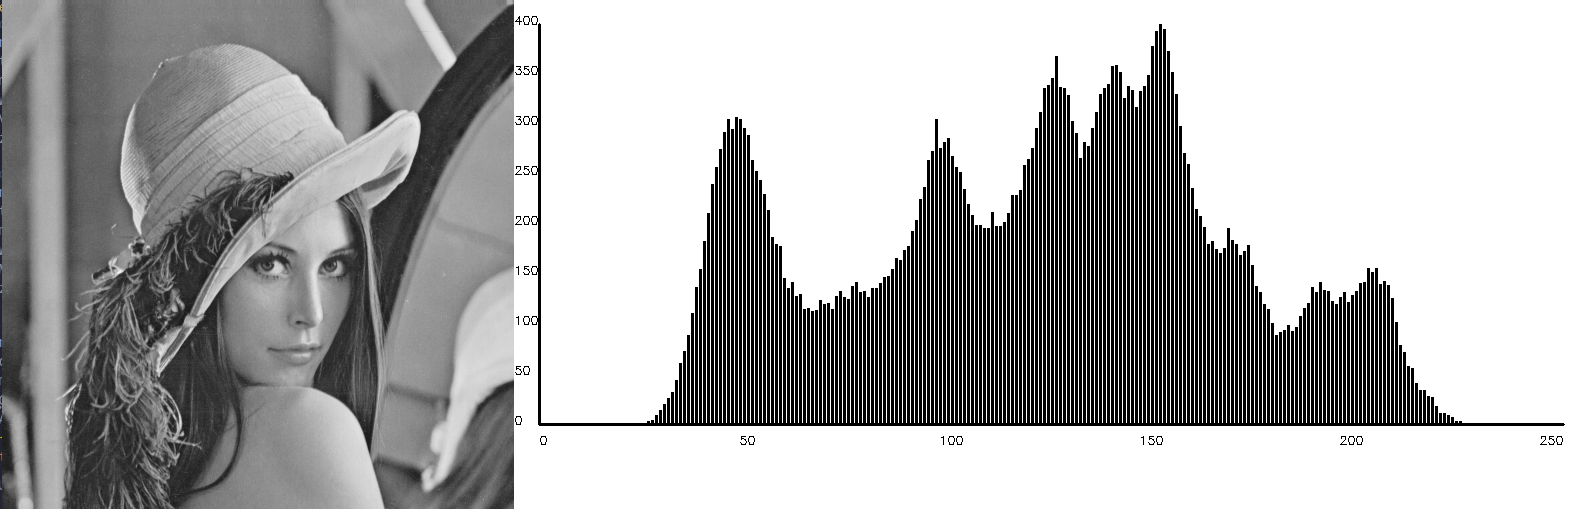
\includegraphics[width=0.8\linewidth]{lena_gsh.png}
        \caption{Grayscale image and its corresponding intensity histogram.\\
        Time taken to calculate the histogram 47 ms}
        \label{fig:gsh}
    \end{figure}
    \item Applying a Gaussian blur with different kernel sizes demonstrated that larger kernels resulted in more pronounced smoothing, at the cost of losing fine details.
    \begin{itemize}
        \item MSE values increased with larger kernel sizes, indicating a greater difference between the original and blurred images.
        \item PSNR values decreased with larger kernel sizes, reflecting the quality loss introduced by the blur.
    \end{itemize}
    
    \begin{figure}[H]
        \centering
        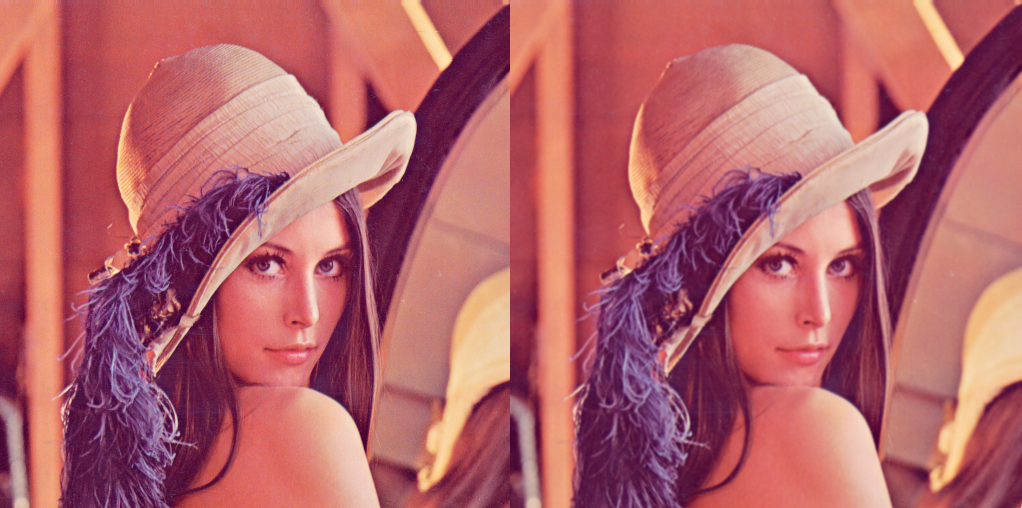
\includegraphics[width=0.5\linewidth]{lena_gf3.png}
        \caption{original image compared to applied GaussianBlur with kernelsize 3, very minor difference.\\
        Time taken to calculate gaussian blur: 45 ms\\
        MSE: 22.9285 \\
        PSNR: 33.147 dB}
        \label{fig:gf3}
    \end{figure}
    \begin{figure}[H]
        \centering
        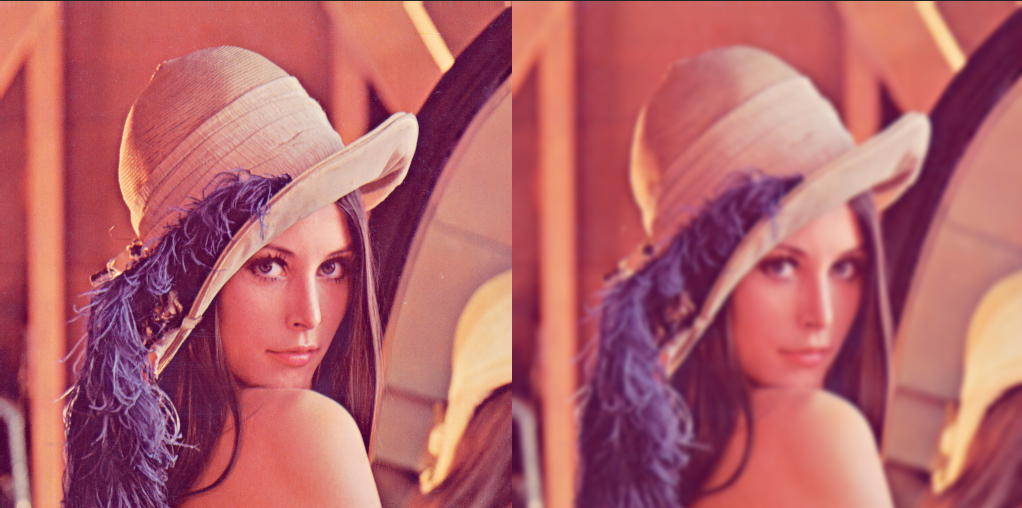
\includegraphics[width=0.5\linewidth]{lena_gf13.png}
        \caption{original image compared to applied GaussianBlur with kernelsize 13, noticable difference.\\
        Time taken to calculate gaussian blur: 51 ms \\
        MSE: 114.884 \\
        PSNR: 27.7703 dB}
        \label{fig:gf13}
    \end{figure}
    
    \item The image comparison metrics allowed us to objectively evaluate the effect of each transformation, providing quantitative evidence of the changes observed visually.
    \begin{figure}[H]
        \centering
        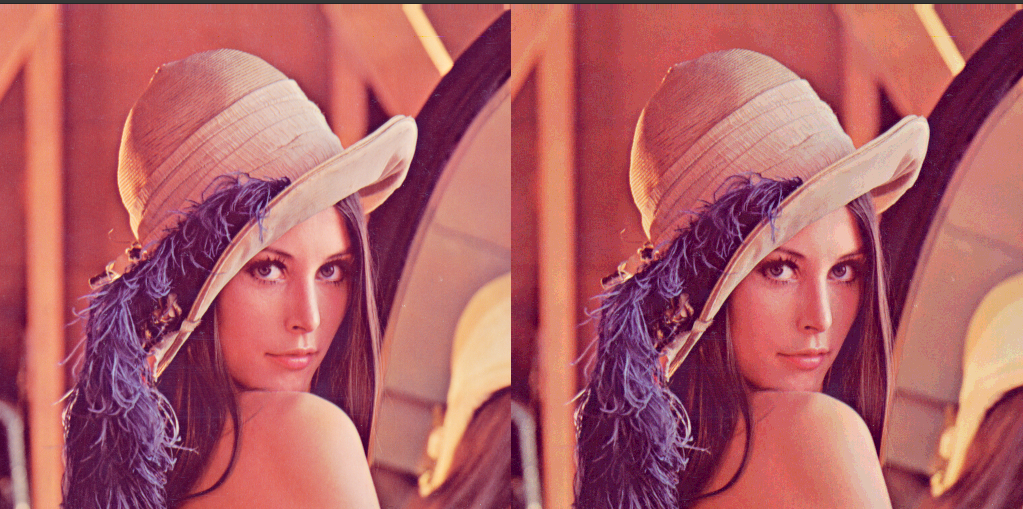
\includegraphics[width=0.5\linewidth]{lena_q.png}
        \caption{original image compared to applied quantized with 16 levels \\
        Time taken to quantize the image 4 ms \\
        MSE: 79.0271 \\
        PSNR: 29.138 dB}
        \label{fig:q}
    \end{figure}
    
\end{itemize}



%\section{Performance Analysis}
%\begin{itemize}
%    \item Processing time for various tasks.
%    \item Trade-offs between quality and compression.
%\end{itemize}

%\section{Discussion}
%\begin{itemize}
%    \item Analysis of outcomes, strengths, and limitations.
%    \item Possible improvements for future work.
%\end{itemize}

\section{Conclusion}
Summarize the key takeaways and learning outcomes from the project.

\section{Appendix}
\begin{itemize}
    \item Link to the project repository: \url{https://github.com/gabrielcosta99/IC-G8.git}
\end{itemize}

\end{document}
